\section{Evaluation}
\label{sec:deepsmith-eval}

\newsavebox{\IntelSizetIntReduced}
\begin{lrbox}{\IntelSizetIntReduced}
  \hspace{1.5em}
  \begin{lstlisting}
    kernel void A(global double* a) {
      int b = get_global_id(0);
      if (b < -1)
        a[b] = 1;
    }
  \end{lstlisting}
\end{lrbox}

\newsavebox{\OclgrindRaceSwitch}
\begin{lrbox}{\OclgrindRaceSwitch}
  \hspace{1.5em}
  \begin{lstlisting}
  kernel void A(global int* a, global int* b) {
    switch (get_global_id(0)) {
    case 0:
      a[get_global_id(0)]=b[get_global_id(0)+13];
      break;
    case 2:
      a[get_global_id(0)]=b[get_global_id(0)+11];
      break;
    case 6:
      a[get_global_id(0)]=b[get_global_id(0)+128];
    }
    barrier(2);
  }
  \end{lstlisting}
\end{lrbox}

\newsavebox{\AlmostEverythingCrash}
\begin{lrbox}{\AlmostEverythingCrash}
  \hspace{1.5em}
  \begin{lstlisting}
    kernel void A() {
      __builtin_astype(d, uint4);
    }
  \end{lstlisting}
\end{lrbox}

\newsavebox{\OclgrindSemaAssertion}
\begin{lrbox}{\OclgrindSemaAssertion}
  \hspace{1.5em}
  \begin{lstlisting}
    kernel void A(global unsigned char* a, global unsigned char* b) {
      unsigned long c = get_global_id(0);
      d[0] = (mad24(f, (int)(a[0], b[get_global_id(0)])) % (d * (d + 3)) + (c / 2))] * a[c + 1];
    }
  \end{lstlisting}
\end{lrbox}
% This has been forwarded to the LLVM folks https://bugs.llvm.org/show_bug.cgi?id=33897
% __kernel void A(__global float* b) {
%	(float4)(b);
% }

\newsavebox{\IntelPtrCompilerHang}
\begin{lrbox}{\IntelPtrCompilerHang}
  \hspace{1.5em}
  \begin{lstlisting}
    kernel void A(global ulong* a) {
      a[get_global_id(0)] = (ulong)(a + 1);
    }
  \end{lstlisting}
\end{lrbox}
% Another 3± hang:
% kernel void A(global const char* a, global char* b, global char* c) {
%   int d = get_global_id(0);
%   c[d] = get_global_id(0) + c;
% }

% Another 3± hang:
% __kernel void A(global int* a) {
%   local int b[4][3][4][5];
%   b[1][2][3][3] = b[3];
% }

\newsavebox{\NvidiaOptLoopHang}
\begin{lrbox}{\NvidiaOptLoopHang}
  \hspace{1.5em}
  % CLgenProgram.id = 6992
  \begin{lstlisting}
    kernel void A(global float* a, global float* b,
                  global float* c) {
      int d, e, f;
      d = get_local_id(0);
      for (int g = 0; g < 100000; g++)
        barrier(1);
    }
  \end{lstlisting}
\end{lrbox}

\newsavebox{\XeonPhiSpin}
\begin{lrbox}{\XeonPhiSpin}
  \hspace{1.5em}
  \begin{lstlisting}
    kernel void A(global unsigned char* a,
                  unsigned b) {
      a[get_global_id(0)] %= 42;
      barrier(1);
    }
  \end{lstlisting}
\end{lrbox}
% LLVM ERROR: LLVM2PIL: Cannot yet select: 0x7f72a45a7ed0: i8,i8 = umul_lohi 0x7f72a45a87d0, 0x7f72a45a88d0 [ORD=16] [ID=22]
% 0x7f72a45a87d0: i8 = srl 0x7f72a45a7dd0, 0x7f72a42fff90 [ORD=16] [ID=21]
% 0x7f72a45a7dd0: i8,ch = load 0x7f72a41d9438, 0x7f72a4300790, 0x7f72a4300590<LD1[%scevgep2]> [ORD=15] [ID=20]
% 0x7f72a4300790: i64 = add 0x7f72a45a83d0, 0x7f72a45a80d0 [ORD=14] [ID=17]
% 0x7f72a45a83d0: i64,ch = CopyFromReg 0x7f72a41d9438, 0x7f72a45a86d0 [ORD=14] [ID=13]
% 0x7f72a45a86d0: i64 = Register %vreg1 [ID=1]
% 0x7f72a45a80d0: i64,ch = CopyFromReg 0x7f72a41d9438, 0x7f72a45a81d0 [ORD=14] [ID=14]
% 0x7f72a45a81d0: i64 = Register %vreg2 [ID=2]
% 0x7f72a4300590: i64 = undef [ID=3]
% 0x7f72a42fff90: i8 = Constant<1> [ID=9]
% 0x7f72a45a88d0: i8 = Constant<49> [ID=10]

\newsavebox{\IntelOptLoopHang}
\begin{lrbox}{\IntelOptLoopHang}
  \hspace{1.5em}
  \begin{lstlisting}
    kernel void A(global int* a) {
      int b = get_global_id(0);
      while (b < 512) { }
    }
  \end{lstlisting}
\end{lrbox}
% Another example:
%   kernel void A(long a, long b) {
%     while (a > 273444) { }
%   }


\newsavebox{\NvidiaRecursionSegfault}
\begin{lrbox}{\NvidiaRecursionSegfault}
  \hspace{1.5em}
  \begin{lstlisting}
    kernel void A(float4 a, global float4* b,
                  global float4* c, unsigned int d,
                  global double* e, global int2* f, 
                  global int4* g, constant int* h, 
                  constant int* i) {
      A(a, b, c, d, d, e, f, g, h);
    }
  \end{lstlisting}
\end{lrbox}
% HAND REDUCED:
%
%   kernel void A(constant int2* a, global int* b) { A(b, a); }
\newsavebox{\NvidiaRecursionSegfaultReduced}
\begin{lrbox}{\NvidiaRecursionSegfaultReduced}
  \hspace{1.5em}
  \begin{lstlisting}
    kernel void B(constant int2* a, global int* b) {
      A(b, a);
    }
  \end{lstlisting}
\end{lrbox}

\newsavebox{\BeignetScalarizeInsert}
\begin{lrbox}{\BeignetScalarizeInsert}
  \hspace{1.5em}
  \begin{lstlisting}
    kernel void A(global float4* a) {
      a[get_local_id(0) / 8][get_local_id(0)] = 
          get_local_id(0);
    }
  \end{lstlisting}
\end{lrbox}

\newsavebox{\OclgrindUncorrectedTypos}
\begin{lrbox}{\OclgrindUncorrectedTypos}
  \hspace{1.5em}
  \begin{lstlisting}
    kernel void A(global float* a, global float* b) {
      a[0] = max(a[c], b[2]);
    }
  \end{lstlisting}
\end{lrbox}

\newsavebox{\BeignetPtrIntSpin}
\begin{lrbox}{\BeignetPtrIntSpin}
  \hspace{1.5em}
  \begin{lstlisting}
    kernel void A(global int* a) {
      int b = get_global_id(0);
      a[b] = (6 * 32) + 4 * (32 / 32) + a;
    }
  \end{lstlisting}
\end{lrbox}

\newsavebox{\NvidiaCompileSegfault}
\begin{lrbox}{\NvidiaCompileSegfault}
  \hspace{1.5em}
  \begin{lstlisting}
    kernel void A(global float* a, local float* b, local float* c, int d, int e) {
      int f, g;
      int h = get_local_id(0);
      int i = get_local_id(1);
      int j = get_global_id(0);
      global char* k = c + f * g + f;
      if (f + 1 < h)
        b[f * d + g * h + g] = g * f;
    }
  \end{lstlisting}
\end{lrbox}

\newsavebox{\XeonPhiSegfault}
\begin{lrbox}{\XeonPhiSegfault}
  \hspace{1.5em}
  \begin{lstlisting}
    kernel void A(void) {
      global int* a;
      unsigned int* b;
      b = a[0];
      a[0] = b;
      a[0] = b;
      barrier(1);
      if (get_global_id(0) == 0)
        *a = 0;
      a[get_local_id(0)] = 0;
    }
  \end{lstlisting}
\end{lrbox}

\newsavebox{\IntelVectorizerSegfault}
\begin{lrbox}{\IntelVectorizerSegfault}
  \hspace{1.5em}
  \begin{lstlisting}
    kernel void A() {
      while (true) {
        barrier(1);
      }
    }
  \end{lstlisting}
\end{lrbox}

\newsavebox{\IntelSizetIntUnreduced}
\begin{lrbox}{\IntelSizetIntUnreduced}
  \hspace{1.5em}
  \begin{lstlisting}
    kernel void A(global double* a, global double* b,
                  global double* c, int d, int e) {
      double f;
      int g = get_global_id(0);
      if (g < e - d - 1)
        c[g] = (((e) / d) % 5) % (e + d);
    }
  \end{lstlisting}
\end{lrbox}

\newsavebox{\PoclUndefinedSymbols}
\begin{lrbox}{\PoclUndefinedSymbols}
  \hspace{1.5em}
  \begin{lstlisting}
    kernel void A(local int* a) {
      for (int b = 0; b < 100; b++)
        B(a);
    }
  \end{lstlisting}
\end{lrbox}


\newsavebox{\BeignetCastError}
\begin{lrbox}{\BeignetCastError}
  \hspace{1.5em}
  \begin{lstlisting}
    kernel void A(global float* a, global float* b, global float* c, const int d) {
      int e = get_global_id(0);
      if (e < d)
        c[e] = a[e] + b[e];
      b[e] = (char)(c[e] + d);
    }
  \end{lstlisting}
\end{lrbox}

\newsavebox{\XeonPhiInvalidWrite}
\begin{lrbox}{\XeonPhiInvalidWrite}
  \hspace{1.5em}
  \begin{lstlisting}
    kernel void A(global int* a) {
      a[0] = 1;
      a[-1] = 2;
      a[0] = 3;
    }
  \end{lstlisting}
\end{lrbox}

\newsavebox{\UninitRead}
\begin{lrbox}{\UninitRead}
  \hspace{1.5em}
  \begin{lstlisting}
      kernel void A(global int* a, global int* b) {
        int c[16];
        int d = get_global_id(0);
        a[d] = b[d] + c[d];
      }
  \end{lstlisting}
\end{lrbox}

\newsavebox{\IntelPtrAssertion}
\begin{lrbox}{\IntelPtrAssertion}
  \hspace{1.5em}
  \begin{lstlisting}
    kernel void A(global int* a, global int* b) {
      int c = (int)get_global_id(0);
      a[c] += b;
    }
  \end{lstlisting}
\end{lrbox}

\newsavebox{\IntelScalarAssertion}
\begin{lrbox}{\IntelScalarAssertion}
  \hspace{1.5em}
  \begin{lstlisting}
    kernel void A(global float* a, global float* b, global float* c, local float* d, unsigned int e, unsigned int f) {
      for (unsigned int g = get_local_id(0) + get_local_size(0); g < get_local_size(0); g += get_local_size(0))
        a[2 * get_local_id(0) + 1] = get_local_id(0);
    }
  \end{lstlisting}
\end{lrbox}

\newsavebox{\BeignetTernary}
\begin{lrbox}{\BeignetTernary}
  \hspace{1.5em}
  \begin{lstlisting}
    kernel void A(global int* a, global int* b, 
                  global int* c) {
      c[0] = (a[0] > b[0]) ? a[0] : 0;
      c[2] = (a[3] <= b[3]) ? a[4] : b[5];
      c[4] = (a[4] <= b[5]) ? a[7] : b[7];
      c[7] = (a[7] < b[0]) ? a[0] : (a[0] > b[1]);
    }
  \end{lstlisting}
\end{lrbox}
% HAND REDUCED:
%
%   kernel void A(global int* a, global int* b, global int* c) {
%     c[0] = 100;
%     c[1] = (a[3] <= b[4]) ? a[4] : b[5];
%   }

\newsavebox{\BeignetTernarySmaller}
\begin{lrbox}{\BeignetTernarySmaller}
  \hspace{1.5em}
  \begin{lstlisting}
    kernel void A(global int* a, global int* b, global int* c) {
      c[0] = (a[0] > 0) ? a[0] : b[1];
      c[1] = (a[1] <= b[1]) ? a[0] : b[0];
    }
  \end{lstlisting}
\end{lrbox}

\newsavebox{\IntelGtDoubleAssertion}
\begin{lrbox}{\IntelGtDoubleAssertion}
  \hspace{1.5em}
  \begin{lstlisting}
    kernel void A(read_only image2d_t a, 
                  global double2* b) {
      b[0] = get_global_id(0);
    }
  \end{lstlisting}
\end{lrbox}

\newsavebox{\IntelDeclDoesntDeclareAnything}
\begin{lrbox}{\IntelDeclDoesntDeclareAnything}
  \hspace{1.5em}
  \begin{lstlisting}
    kernel void A() {
      char a;
      int b;
      int const;
    }
  \end{lstlisting}
\end{lrbox}

\newsavebox{\AddressQualifiedAutoVar}
\begin{lrbox}{\AddressQualifiedAutoVar}
  \hspace{1.5em}
  \begin{lstlisting}
    kernel void A(global float4* a, global float4* b, global float4* c, global float4* d, global float4* e, float f) {
      unsigned int g = get_global_id(0);
      int h = get_global_size(0);
      constant sampler_t i = 0x0000 | 0x0004 | 0x0000;
      unsigned int j = g * (1 << ((h % 4) - (2)));
    }
  \end{lstlisting}
\end{lrbox}

\newsavebox{\NvidiaLocalGlobalSegfault}
\begin{lrbox}{\NvidiaLocalGlobalSegfault}
  \hspace{1.5em}
  \begin{lstlisting}
    kernel void A(global int* a) {
      local int b[2][3][4][5];
      if (get_global_id(0) == 0)
        a = b[0];
    }
  \end{lstlisting}
\end{lrbox}

\newsavebox{\NvidiaLocalSegfault}
\begin{lrbox}{\NvidiaLocalSegfault}
  \hspace{1.5em}
  \begin{lstlisting}
    kernel void A(global uchar4* a, const int b) {
      local int c[16];
      local float8* d = a + 133;
      atomic_cmpxchg(c, 10, 13);
    }
  \end{lstlisting}
\end{lrbox}


% Program ID: 35612
\newsavebox{\IntelPostDominanceFrontier}
\begin{lrbox}{\IntelPostDominanceFrontier}
  \hspace{1.5em}
  \begin{lstlisting}
    kernel void A() {
      while (true)
        barrier(1);
    }
  \end{lstlisting}
\end{lrbox}
% Another:
% kernel void A(local int* a) {
%   while (1) {
%   }
% }
%
% And another:
%    kernel void A(global int* a) {
%      bool b;
%      int c;
%      for (b = 0; b < 100; b++)
%        a[c] += a[c];
%    }
%
% One more:
%   kernel void A(global int* a, global int* b) {
%     int c = get_global_id(0);
%     int d = 0;
%     while (d < 1024)
%       a[c] = d;
%   }

\newsavebox{\IntelPredicator}
\begin{lrbox}{\IntelPredicator}
  \hspace{1.5em}
  \begin{lstlisting}
    kernel void A(global int* a) {
      int b = get_global_id(0);
      while (b < *a)
        if (a[0] < 0)
          a[1] = b / b * get_local_id(0);
    }
  \end{lstlisting}
\end{lrbox}

\newsavebox{\IntelPrepareKernelArgs}
\begin{lrbox}{\IntelPrepareKernelArgs}
  \hspace{1.5em}
  \begin{lstlisting}
    kernel void A(int a, global int* b) {
      int c = get_global_id(0);
      int d = work_group_scan_inclusive_max(c);
      b[c] = c;
    }
  \end{lstlisting}
\end{lrbox}

\newsavebox{\IntelDAGInstrSelection}
\begin{lrbox}{\IntelDAGInstrSelection}
  \hspace{1.5em}
  \begin{lstlisting}
    kernel void A(global half* a, global int* b, global bool* c, int d, int e) {
      int f = get_global_id(0);
      int g = get_global_id(1) * e;
      if (f < e)
        a[f] = b[f];
    }
  \end{lstlisting}
\end{lrbox}

\newsavebox{\IntelSPIRMetadata}
\begin{lrbox}{\IntelSPIRMetadata}
  \hspace{1.5em}
  \begin{lstlisting}
    kernel void A() {
      local float a; A(a);
    }
  \end{lstlisting}
\end{lrbox}

\newsavebox{\IntelRemoveDupeBarrier}
\begin{lrbox}{\IntelRemoveDupeBarrier}
  \hspace{1.5em}
  \begin{lstlisting}
    kernel void A() {
      local int a[10];
      local int b[16][16];
      a[1024 + (2 * get_local_id(1) +
        get_local_id(0)) + get_local_id(0)] = 6;
      barrier(b);
    }
  \end{lstlisting}
\end{lrbox}

\newsavebox{\IntelCombineRedundant}
\begin{lrbox}{\IntelCombineRedundant}
  \hspace{1.5em}
  \begin{lstlisting}
    kernel void A(global float* a, global float* b,
                  global float* c, const int d) {
      for (unsigned int e = get_global_id(0);
           e < d; e += get_global_size(0))
        for (unsigned f = 0; f < d; ++f)
          e += a[f];
    }
  \end{lstlisting}
\end{lrbox}


\newsavebox{\BeigPtrAssertion}
\begin{lrbox}{\BeigPtrAssertion}
  \hspace{1.5em}
  \begin{lstlisting}
    kernel void A(global int* a, global int* b,
                  global int* c) {
      a[get_global_id(0)] = a[get_global_id(0)] > b;
    }
  \end{lstlisting}
\end{lrbox}

\newsavebox{\BeigIterAssertion}
\begin{lrbox}{\BeigIterAssertion}
  \hspace{1.5em}
  \begin{lstlisting}
    kernel void A(global int* a) {
      global int* b = ((void*)0);
      b[0] = a;
    }
  \end{lstlisting}
\end{lrbox}

\newsavebox{\ParserFailOne}
\begin{lrbox}{\ParserFailOne}
  \hspace{1.5em}
  \begin{lstlisting}
    void A(){(global a*)()
  \end{lstlisting}
\end{lrbox}

\newsavebox{\ParserFailTwo}
\begin{lrbox}{\ParserFailTwo}
  \hspace{1.5em}
  \begin{lstlisting}
    void A(){void* a; uint4 b=0; b=(b>b)?a:a
  \end{lstlisting}
\end{lrbox}

\newsavebox{\ParserFailThree}
\begin{lrbox}{\ParserFailThree}
  \hspace{1.5em}
  \begin{lstlisting}
    void A(){double2 k; return (float4)(k,k,k,k)
  \end{lstlisting}
\end{lrbox}

\newsavebox{\DagPass}
\begin{lrbox}{\DagPass}
  \hspace{1.5em}
  \begin{lstlisting}
    kernel void A(global half* a) {
      int b = get_global_id(0);
      a[b] = b * b;
    }
  \end{lstlisting}
\end{lrbox}

\newsavebox{\SimplifyTheCFGPass}
\begin{lrbox}{\SimplifyTheCFGPass}
  \hspace{1.5em}
  \begin{lstlisting}
    kernel void A(global float* a, global float* b,
                  const int c) {
      for (int d = 0; d < c; d++)
        for (d = 0; d < a; d += 32)
          b[d] = 0;
    }
  \end{lstlisting}
\end{lrbox}

\newsavebox{\LoopWIAnalysisPass}
\begin{lrbox}{\LoopWIAnalysisPass}
  \hspace{1.5em}
  \begin{lstlisting}
    kernel void A(global int* a, const int b, const int c) {
      int d; int e; int f = 0;
      for (int g = b >> 1; g > 1; g >>= 1) {
        barrier(1);
        for (int h = c; h < g; h += d) {
          int i = f * (2 * h + 1) - 1;
          int j = f * (2 * h + 2) - 1;
          a[j] += a[i];
        }
      }
    }
  \end{lstlisting}
\end{lrbox}

This section reports on the results of DeepSmith testing of the 10 OpenCL systems from Table~\ref{tab:deepsmith-platforms}, in which each ran for 48 hours. Bugs were found in all the compilers tested --- every compiler crashed, and every compiler generated programs which either crash or silently compute the wrong result. To date, 67 unique bug reports have been submitted to compiler vendors. This section first contains a qualitative analysis of compile-time and runtime defects found, followed by a quantitative comparison of the approach against the state-of-the-art in OpenCL compiler fuzzing --- CLSmith~\cite{Lidbury2015a}. DeepSmith is able to identify a broad range of defects, many of which CLSmith cannot, for only a fraction of the engineering effort. Finally, this section contains a quantitative analysis of compiler robustness over time, using the compiler crash rate of every LLVM release in the past two years as a metric of compiler robustness. The findings show that progress is good, compilers are becoming more robust, yet the introduction of new features and regressions ensures that compiler validation remains a moving target.

Unless stated otherwise, DeepSmith code listings are presented verbatim, with only minor formatting changes applied to preserve space. No test case reduction, either manual or automatic, was needed.

For the remainder of this chapter, testbeds are identified using the OpenCL system number from Table~\ref{tab:deepsmith-platforms}, suffixed with $+$, $-$, or $\pm$ to denote optimisations on, off, or either, respectively.

\subsection{Compile-time Defects}%
\label{subsec:compile-time-defects}

OpenCL is typically compiled online, which amplifies the significance of detecting compile-time defects, as they may not be discovered until code has been shipped to customers. Numerous cases were found where DeepSmith kernels trigger a crash in the compiler (and as a result, the host process), or cause the compiler to loop indefinitely. In the testing time allotted 199 test cases were identified which trigger unreachable code failures, triggered 31 different compiler assertions, and produced 114 distinct stack traces from other compiler crashes.

\begin{figure}
  \centering %
  \subfloat[Reduced from 48 line kernel.]{%
  \noindent\mbox{\parbox{\columnwidth}{\usebox{\ParserFailOne}}}%
  }\\%
  \subfloat[Reduced from 52 line kernel.]{%
  \noindent\mbox{\parbox{\columnwidth}{\usebox{\ParserFailTwo}}}%
  }\\%
  \subfloat[Reduced from 68 line kernel.]{%
  \noindent\mbox{\parbox{\columnwidth}{\usebox{\ParserFailThree}}}%
  }\\%
  \caption[Example codes which crash parsers]{%
    Example codes which crash OpenCL compilers during parsing.%
  }%
  \label{lst:parser-crashes}
  %
\end{figure}

\subsubsection{Semantic Analysis Failures}

Compilers should produce meaningful diagnostics when inputs are invalid, yet dozens of compiler defects were discovered attributable to improper or missing error handling. Many generation and mutation based approaches to compiler validation have focused solely on testing under \emph{valid inputs}. As such, this class of bugs may go undiscovered. Compared to these approaches, DeepSmith may contribute a significant improvement for generating plausibly-erroneous code over prior random-enumeration approaches.

The use of undeclared identifiers is a core error diagnostic which one would expect to be robust in a mature compiler. DeepSmith discovered cases in which the presence of undeclared identifiers causes the Testbeds $10\pm$ compiler to crash. For example, the undeclared identifier \texttt{c} in Figure~\ref{lst:oclgrind-uncorrected-typos} raises an assertion during semantic analysis of the AST when used as an array index.

\begin{figure}
  \centering %
  \subfloat[Testbeds $10\pm$ assertion \emph{Uncorrected typos!} during semantic analysis.]{%
    \noindent\mbox{\parbox{\columnwidth}{\usebox{\OclgrindUncorrectedTypos}}}%
    \label{lst:oclgrind-uncorrected-typos}
  }\\%
  \subfloat[Testbeds $1\pm$, $2\pm$ segmentation fault due to implicit address space conversion.]{%
    \noindent\mbox{\parbox{\columnwidth}{\usebox{\NvidiaRecursionSegfault}}}%
    \label{lst:nvidia-recursion-segfault}
  }\\%
  \subfloat[Testbeds $3\pm$ assertion \emph{sel.hasDoubleType()} during code generation.]{%
    \noindent\mbox{\parbox{\columnwidth}{\usebox{\IntelGtDoubleAssertion}}}%
    \label{lst:intel-gt2-double-assertion}
  }\\%
  \subfloat[Testbeds $3\pm$ assertion \emph{scalarizeInsert} during code generation.]{%
    \noindent\mbox{\parbox{\columnwidth}{\usebox{\BeignetScalarizeInsert}}}%
    \label{lst:beignet-scalarize-insert}
  }\\%
  \subfloat[Of the 10 compilers we tested, 6 crash with segfault when compiling this kernel.]{%
    \noindent\mbox{\parbox{\columnwidth}{\usebox{\AlmostEverythingCrash}}}%
    \label{lst:almost-everything-crash}
  }\\%
  \caption[Example OpenCL kernels which crash compilers]{%
    Example OpenCL kernels which crash compilers.%
  }%
\end{figure}

Type errors were an occasional cause of compile-time defects. Figure~\ref{lst:nvidia-recursion-segfault} induces a crash in NVIDIA compilers due to an implicit conversion between global to constant address qualifiers. Worse, Testbeds $3\pm$ were found to loop indefinitely on some kernels containing implicit conversions from a pointer to an integer, as shown in Figure~\ref{lst:beignet-ptr-int-spin}. While spinning, the compiler would utilise 100\% of the CPU and consume an increasing amount of host memory until the entire system memory is depleted and the process crashes.

Occasionally, incorrect program semantics will remain undetected until late in the compilation process. Both Figures~\ref{lst:intel-gt2-double-assertion} and~\ref{lst:beignet-scalarize-insert} pass the type checker and semantic analysis, but trigger compiler assertions during code generation.

An interesting yet unintended by-product of having trained DeepSmith on thousands of real-world examples is that the model learned to occasionally generate compiler-specific code, such as invoking compiler intrinsics. The quality of error handling on these builtins was found to vary wildly. For example, Figure~\ref{lst:almost-everything-crash} silently crashes 6 of the 10 compilers, which, to the best of my knowledge, makes DeepSmith the first random program generator to induce a defect through exploiting compiler-specific functionality.

\subsubsection{Parser Failures}

Parser development is a mature and well-understood practice. Still, parser errors were discovered in several compilers. Each of the code samples in Figure~\ref{lst:parser-crashes} induce crash errors during parsing of compound statements in both Testbeds $5\pm$ and $7\pm$. For space, the listings have been hand-reduced to minimal code samples, which have been reported to Intel. Each reduction took around 6 edit-compile steps, taking less than 10 minutes. In total, 100 distinct programs have been generated which crash compilers during parsing.

\begin{figure}
  \centering %
  \subfloat[Testbeds $3\pm$ loop indefinitely, leaking memory until the entire system memory is depleted and the process crashes.]{%
  \noindent\mbox{\parbox{\columnwidth}{\usebox{\BeignetPtrIntSpin}}}%
  \label{lst:beignet-ptr-int-spin}
  }\\%
  \subfloat[Testbed $1+$ hangs during optimisation of kernels with large loop bounds. Testbeds $1-$ and $2\pm$ compile in under 1 second.]{%
  \noindent\mbox{\parbox{\columnwidth}{\usebox{\NvidiaOptLoopHang}}}%
  \label{lst:nvidia-opt-loop-hang}
  }\\%
  \subfloat[Testbeds $7\pm$ loops indefinitely, consuming 100\% CPU usage.]{%
	\noindent\mbox{\parbox{\columnwidth}{\usebox{\XeonPhiSpin}}}%
	\label{lst:xeon-phi-spin}
  }\\%
  \subfloat[Testbeds $4+$, $5+$, $6+$, $7+$ hang during optimisation of kernels with non-terminating loops.]{%
  \noindent\mbox{\parbox{\columnwidth}{\usebox{\IntelOptLoopHang}}}%
  \label{lst:intel-inf-loop}
  }\\%
  \caption[Example kernels which hang compilers]{%
    Example OpenCL kernels which hang compilers.%
  }%
  \label{lst:compiler-hangs}
\end{figure}

\subsubsection{Compiler Hangs}

As expected, some compile-time defects are optimisation sensitive. Testbed $1+$ hangs on large loop bounds, shown in Figure~\ref{lst:nvidia-opt-loop-hang}. All commercial Intel compilers  tested hang during optimisation of non-terminating loops (Figure~\ref{lst:intel-inf-loop}).

Testbeds $7\pm$ loop indefinitely during compilation of the simple OpenCL kernel in Figure~\ref{lst:xeon-phi-spin}.

\subsubsection{Other errors}

Some compilers are more permissive than others. Testbeds~$4\pm$, $6\pm$, $9\pm$ reject out-of-range literal values e.g. \texttt{int i = 0xFFFFFFFFFFFFFFFFFFFFFFFF}, whilst Testbeds $3\pm$, $5\pm$, $7\pm$, $8\pm$, and $10\pm$ interpret the literal as an \texttt{unsigned long long} and implicitly cast to an integer value of \texttt{-1}. Testbeds $1\pm$, $2\pm$ emit no warning.

Testbeds~$1\pm$, $2\pm$, $3\pm$ rejected address space qualifiers on automatic variables, where all other testbeds successfully compiled and executed.

On Testbeds~$3\pm$, the statement \texttt{int n = mad24(a, (32), get\_global\_size(0));} (a call to a maths builtin with mixed types) is rejected as ambiguous.


\subsection{Runtime Defects}

Prior work on compiler test case generation has focused on extensive stress-testing of compiler middle-ends to uncover miscompilations~\cite{Chen2014a}. CSmith, and by extension, CLSmith, specifically targets this class of bugs. Grammar-based enumeration is highly effective at this task, yet is bounded by the expressiveness of the grammar. Here, examples are provided of bugs which cannot currently be discovered by CLSmith.


\subsubsection{Thread-dependent Flow Control}

A common pattern in OpenCL is to obtain the thread identity, often as an \texttt{int}, and to compare this against some fixed value to determine whether or not to complete a unit of work (46\% of OpenCL kernels on GitHub use this ($tid \rightarrow$ int, \texttt{if (tid < \ldots) \{\ldots\}}) pattern). DeepSmith, having modelled the frequency with which this pattern occurs in real handwritten code, generates many permutations of this pattern. And in doing so, exposed a bug in the optimiser of Testbeds $4+$ and $6+$ which causes the \texttt{if} branch in Figure~\ref{lst:intel-size_t-int-unreduced} to be erroneously executed when the kernel is compiled with optimisations enabled. This issue has been reported to Intel. CLSmith does not permit the thread identity to modify control flow, rendering such productions impossible.

\begin{figure}
  \centering %
  \subfloat[Testbeds $4+$, $6+$ incorrectly optimise the \texttt{if} statement, causing the conditional branch to execute (it shouldn't). This pattern of integer comparison to thread ID is widely used.]{%
    \noindent\mbox{\parbox{\columnwidth}{\usebox{\IntelSizetIntUnreduced}}}%
    \label{lst:intel-size_t-int-unreduced}
  }\\%
  \subfloat[A race condition in \texttt{switch} statement evaluation causes $10\pm$ to sporadically crash when executed with a number of threads $> 1$.]{%
    \noindent\mbox{\parbox{\columnwidth}{\usebox{\OclgrindRaceSwitch}}}%
    \label{lst:oclgrind-race-switch}
  }\\%
  \subfloat[Testbeds $3\pm$ silently miscompile ternary assignments in which the operands are different global buffers.]{%
    \noindent\mbox{\parbox{\columnwidth}{\usebox{\BeignetTernary}}}%
    \label{lst:beig-ternary-ops}
  }\\%
  \caption[Example kernels which are miscompiled]{%
    Example OpenCL kernels which are miscompiled.%
  }%
\end{figure}

\begin{figure}
  \centering %
  \subfloat[Compilation should fail due to call to undefined function \texttt{B()}; Testbeds $8\pm$ silently succeed then crash upon kernel execution.]{%
    \noindent\mbox{\parbox{\columnwidth}{\usebox{\PoclUndefinedSymbols}}}%
    \label{lst:pocl-undefined-symbols}
  }\\%
  \caption[Further example kernel which is miscompiled]{%
    Further example OpenCL kernel which is miscompiled.%
  }%
\end{figure}

Figure~\ref{lst:oclgrind-race-switch} shows a simple program in which thread identity determines the program output. This test case was found to sporadically crash Testbeds~$10\pm$, an OpenCL device simulator and debugger. Upon reporting to the developers, the underlying cause was quickly diagnosed as a race condition in \texttt{switch} statement evaluation and fixed within a week.


\subsubsection{Kernel Inputs}

CLSmith kernels accept a single buffer parameter into which each thread computes its result. This fixed prototype limits the ability to detect bugs which depend on input arguments. Figure~\ref{lst:beig-ternary-ops} exposes a bug of this type. Testbeds $3\pm$ will silently miscompile ternary operators when the ternary operands consist of values stored in multiple different global buffers. CLSmith, with its fixed single input prototype, is unable to discover this bug.


\subsubsection{Latent Compile-time Defects}

Sometimes, invalid compiler inputs may go undetected, leading to runtime defects only upon program execution. Since CLSmith enumerates only well-formed programs, this class of bugs cannot be discovered.

Figure~\ref{lst:pocl-undefined-symbols} exposes a bug in which a kernel containing an undefined symbol will successfully compile without warning on Testbeds~$8\pm$, then crash the program when attempting to run the kernel. This issue has been reported to the developers and fixed.


\subsection{Comparison to State-of-the-art}

This section provides a quantitative comparison of the bug-finding capabilities of DeepSmith and CLSmith.


\subsubsection{Results Overview}

Tables~\ref{tab:megatable-clsmith} and~\ref{tab:megatable-deepsmith} shows the results of 48 hours of consecutive testing for all Testbeds using CLSmith and DeepSmith, respectively. An average of 15k CLSmith and 91k DeepSmith test cases were evaluated on each Testbed, taking 12.1s and 1.90s per test case respectively. There are three significant factors providing the sixfold increase in testing throughput achieved by DeepSmith over CLSmith: test cases are faster to generate, test cases are less likely to timeout (execute for 60 seconds without termination), and the test cases which do not timeout execute faster.

\begin{table}
	\centering %
	\caption[Results from 48 hours of testing using CLSmith]{%
		Results from 48 hours of testing using CLSmith. System \#. as per Table~\ref{tab:deepsmith-platforms}. $\pm$ denotes optimisations off ($-$) vs on ($+$). The remaining columns denote the number of build crash (\bc), build timeout (\bto), anomalous build failure (\abf), anomalous runtime crash (\arc), anomalous wrong-output (\awo), and pass (\textbf{\cmark}) results.
	}
	\begin{tabular}{| lll | rrrrrrr |}
  \hline
  \rowcolor{gray!50}
  \textbf{\#.} & \textbf{Device} & $\pm$ &
  \bc & \bto & \abf & \arc & \awo & \textbf{\cmark} & \textbf{total} \\
  \hline
  & & $-$ & 0 & 0 & 0 & 2 & 2 & 15628 & 15632  \\
  \multirow{ -2}{*}{1} & \multirow{-2}{*}{GeForce GTX 1080} & $+$ & 0 & 71 & 0 & 6 & 9 & 14007 & 14093 \\
  \rowcolor{gray!25}
  & & $-$ & 0 & 0 & 0 & 28 & 5 & 18220 & 18253 \\
  \rowcolor{gray!25}
  \multirow{-2}{*}{2} & \multirow{-2}{*}{GeForce GTX 780} & $+$ & 26 & 14 & 0 & 0 & 3 & 17654 & 17697 \\
  & & $-$ & 2714 & 2480 & 0 & 0 & 3 & 1121 & 6318 \\
  \multirow{-2}{*}{3} & \multirow{-2}{*}{Intel HD Haswell GT2} & $+$ & 2646 & 2475 & 0 & 0 & 3 & 1075 & 6199 \\
  \rowcolor{gray!25}
  & & $-$ & 0 & 27 & 1183 & 0 & 0 & 16313 & 17523 \\
  \rowcolor{gray!25}
  \multirow{-2}{*}{4} & \multirow{-2}{*}{Intel E5-2620 v4} & $+$ & 487 & 87 & 1130 & 0 & 0 & 17350 & 19054 \\
  & & $-$ & 0 & 11 & 0 & 0 & 0 & 17887 & 17898 \\
  \multirow{-2}{*}{5} & \multirow{-2}{*}{Intel E5-2650 v2} & $+$ & 112 & 175 & 0 & 0 & 0 & 14626 & 14913 \\
  \rowcolor{gray!25}
  & & $-$ & 0 & 14 & 1226 & 0 & 0 & 17118 & 18358 \\
  \rowcolor{gray!25}
  \multirow{-2}{*}{6} & \multirow{-2}{*}{Intel i5-4570} & $+$ & 526 & 63 & 1180 & 0 & 0 & 19185 & 20954 \\
  & & $-$ & 4 & 84 & 0 & 0 & 8 & 13265 & 13361 \\
  \multirow{-2}{*}{7} & \multirow{-2}{*}{Intel Xeon Phi} & $+$ & 42 & 1474 & 0 & 0 & 2 & 3258 & 4776 \\
  \rowcolor{gray!25}
  & & $-$ & 0 & 0 & 0 & 675 & 0 & 17250 & 17925 \\
  \rowcolor{gray!25}
  \multirow{-2}{*}{8} & \multirow{-2}{*}{POCL (Intel E5-2620)} & $+$ & 0 & 3 & 0 & 99 & 5 & 13980 & 14087 \\
  & & $-$ & 0 & 0 & 0 & 0 & 0 & 18479 & 18479 \\
  \multirow{-2}{*}{9} & \multirow{-2}{*}{ComputeAorta} & $+$ & 0 & 0 & 0 & 300 & 11 & 18625 & 18936 \\
  \rowcolor{gray!25}
  & & $-$ & 0 & 0 & 0 & 0 & 0 & 5287 & 5287 \\
  \rowcolor{gray!25}
  \multirow{-2}{*}{10} & \multirow{-2}{*}{Oclgrind Simulator} & $+$ & 0 & 0 & 0 & 0 & 0 & 5334 & 5334 \\
  \hline
\end{tabular}

	\label{tab:megatable-clsmith}
\end{table}

\begin{table}
  \centering %
  \caption[Results from 48 hours of testing using DeepSmith]{%
    Results from 48 hours of testing using DeepSmith. System \#. as per Table~\ref{tab:deepsmith-platforms}. $\pm$ denotes optimisations off ($-$) vs on ($+$). The remaining columns denote the number of build crash (\bc), build timeout (\bto), anomalous build failure (\abf), anomalous runtime crash (\arc), anomalous wrong-output (\awo), and pass (\textbf{\cmark}) results.
  }
  \setlength\extrarowheight{2pt}
\begin{tabular}{| lll | rrrrrrr |}
  \hline
  \rowcolor{gray!50}
  \textbf{\#.} & \textbf{Device} & $\pm$ &
  \bc & \bto & \abf & \arc & \awo & \textbf{\cmark} & \textbf{total} \\
  \hline
  & & $-$ & 27 & 0 & 3 & 0 & 5 & 62105 & 62140 \\
  \multirow{ -2}{*}{1} & \multirow{-2}{*}{GeForce GTX 1080} & $+$ & 20 & 1 & 1 & 0 & 7 & 57361 & 57390 \\
  \rowcolor{gray!25}
  & & $-$ & 27 & 0 & 3 & 0 & 9 & 87129 & 87168 \\
  \rowcolor{gray!25}
  \multirow{-2}{*}{2} & \multirow{-2}{*}{GeForce GTX 780} & $+$ & 32 & 1 & 1 & 0 & 9 & 82666 & 82709 \\
  & & $-$ & 574 & 200 & 2 & 0 & 12 & 136977 & 137765 \\
  \multirow{-2}{*}{3} & \multirow{-2}{*}{Intel HD Haswell GT2} & $+$ & 569 & 200 & 5 & 0 & 10 & 135430 & 136214 \\
  \rowcolor{gray!25}
  & & $-$ & 57 & 0 & 9 & 1 & 0 & 107982 & 108049 \\
  \rowcolor{gray!25}
  \multirow{-2}{*}{4} & \multirow{-2}{*}{Intel E5-2620 v4} & $+$ & 320 & 147 & 7 & 3 & 0 & 113616 & 114093 \\
  & & $-$ & 152 & 2 & 0 & 0 & 0 & 90882 & 91036 \\
  \multirow{-2}{*}{5} & \multirow{-2}{*}{Intel E5-2650 v2} & $+$ & 170 & 117 & 0 & 0 & 1 & 90478 & 90766 \\
  \rowcolor{gray!25}
  & & $-$ & 73 & 0 & 9 & 2 & 1 & 111240 & 111325 \\
  \rowcolor{gray!25}
  \multirow{-2}{*}{6} & \multirow{-2}{*}{Intel i5-4570} & $+$ & 318 & 140 & 7 & 2 & 1 & 117049 & 117517 \\
  & & $-$ & 68 & 4 & 0 & 0 & 1 & 37171 & 37244 \\
  \multirow{-2}{*}{7} & \multirow{-2}{*}{Intel Xeon Phi} & $+$ & 77 & 47 & 0 & 0 & 0 & 37501 & 37625 \\
  \rowcolor{gray!25}
  & & $-$ & 54 & 1 & 2 & 89 & 3 & 85318 & 85467 \\
  \rowcolor{gray!25}
  \multirow{-2}{*}{8} & \multirow{-2}{*}{POCL (Intel E5-2620)} & $+$ & 46 & 0 & 1 & 104 & 4 & 81267 & 81422 \\
  & & $-$ & 51 & 0 & 1 & 3 & 1 & 112324 & 112380 \\
  \multirow{-2}{*}{9} & \multirow{-2}{*}{ComputeAorta} & $+$ & 59 & 0 & 0 & 48 & 4 & 115323 & 115434 \\
  \rowcolor{gray!25}
  & & $-$ & 2081 & 0 & 0 & 0 & 1 & 73261 & 75343 \\
  \rowcolor{gray!25}
  \multirow{-2}{*}{10} & \multirow{-2}{*}{Oclgrind Simulator} & $+$ & 2265 & 0 & 0 & 0 & 0 & 77959 & 80224 \\
  \hline
\end{tabular}

  \label{tab:megatable-deepsmith}
\end{table}

Figure~\ref{fig:deepsmith-vs-clsmith}a shows the generation and execution times of DeepSmith and CLSmith test cases, excluding timeouts\footnote{If timeouts are included then the performance improvement of DeepSmith is $6.5\times$ with the execution times being $11\times$ faster. However, this number grows as the arbitrary timeout threshold is changed, so for fairness timeouts have been excluded.}. DeepSmith generation time grows linearly with program length and is on average $2.45\times$ faster than CLSmith. Test case execution is on average $4.46\times$ faster than CLSmith.

\begin{figure}
  \centering %
  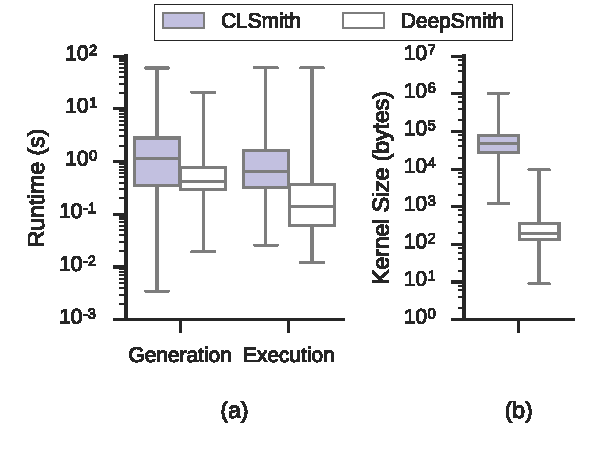
\includegraphics[width=.72\columnwidth]{img/deepsmith-vs-clsmith}%
  \caption[Comparison of DeepSmith and CLSmith runtimes]{%
    Comparison of runtimes (a) and test case sizes (b). DeepSmith test cases are on average evaluated $3.03\times$ faster than CLSmith ($2.45\times$, and $4.46\times$ for generation and execution, respectively), and are two orders of magnitude smaller. Timings do not include the cost of timeouts which would increase the performance gains of DeepSmith by nearly a factor of two.%
  }%
  \label{fig:deepsmith-vs-clsmith}
\end{figure}

The optimisation level generally does not affect testing throughput significantly, with the exception of Testbed~$7+$. Optimisation of large structs is expensive on Testbed~$7+$, and CLSmith test cases use global structs extensively. This is a known issue --- in~\cite{Lidbury2015a} the authors omit large-scale testing on this device for this reason. The use of structs in handwritten OpenCL is comparatively rare --- only 7.1\% of kernels on GitHub use them.


\subsubsection{Comparison of Test Cases}

The average CLSmith program is 1189 lines long (excluding headers). CLSmith test cases require reduction in order to expose the underlying bug. An automated approach to OpenCL test case reduction is presented in~\cite{Pflanzer2016}, though it requires on average 100 minutes for each test case using a parallelised implementation (and over 6 hours if this parallelisation is not available); still, the authors suggest a final manual pass after automated reduction. In contrast, DeepSmith learned to program from humans, and humans do not typically write such large kernel functions. The average DeepSmith kernel is 20 lines long, which is interpretable without reduction, either manual or automatic.


\subsubsection{Comparison of Results}

Both testing systems found anomalous results of all types. In 48 hours of testing, CLSmith discovered compile-time crashes (\bc) in 8 of the 20 testbeds, DeepSmith crashed all of them. DeepSmith triggered 31 distinct compiler assertions, CLSmith 2. Both of the assertions triggered by CLSmith were also triggered by DeepSmith. DeepSmith also triggered 3 distinct \emph{unreachable!} compile-time crashes, CLSmith triggered 0. The ratio of build failures is higher in the token-level generation of DeepSmith (51\%) than the grammar-based generation of CLSmith (26\%).

The Intel CPU Testbeds ($4\pm$, $5\pm$, $6\pm$, and~$7\pm$) would occasionally emit a stack trace upon crashing, identifying the failure point in a specific compiler pass. CLSmith triggered such crashes in 4 distinct passes. DeepSmith triggered crashes in 10 distinct passes, including 3 of the 4 in which CLSmith did. Figures~\ref{lst:intel-passes} and~\ref{lst:further-intel-passes} provide examples. Many of these crashes are optimisation sensitive and are more likely to occur when optimisations are enabled. CLSmith was able to induce a crash in only one of the Intel testbeds with optimisations disabled. DeepSmith crashed all of the compilers with both optimisations enabled and disabled.

\begin{figure}
  \centering
  % Result id: 110876
  \subfloat[\emph{Post-Dominance Frontier Construction} pass.]{%
  \noindent\mbox{\parbox{\columnwidth}{\usebox{\IntelPostDominanceFrontier}}}%
  }\\%
  \subfloat[\emph{Simplify the CFG} pass.]{%
  \noindent\mbox{\parbox{\columnwidth}{\usebox{\SimplifyTheCFGPass}}}%
  }\\%
  % Program id: 31656
  \subfloat[\emph{Predicator} pass.]{%
  \noindent\mbox{\parbox{\columnwidth}{\usebox{\IntelPredicator}}}%
  }\\%
  \subfloat[\emph{Combine redundant instructions} pass.]{%
  \noindent\mbox{\parbox{\columnwidth}{\usebox{\IntelCombineRedundant}}}%
  }\\%
  % Program id: 10596
  \subfloat[\emph{PrepareKernelArgs} pass.]{%
  \noindent\mbox{\parbox{\columnwidth}{\usebox{\IntelPrepareKernelArgs}}}%
  }\\%
  \caption[Example kernels which crash Intel compiler passes]{%
    Example OpenCL kernels which crash Intel compiler passes.%
  }%
  \label{lst:intel-passes}
\end{figure}

\begin{figure}
	\centering
	% Program id: 37443
	\subfloat[\emph{Add SPIR related module scope metadata} pass.]{%
		\noindent\mbox{\parbox{\columnwidth}{\usebox{\IntelSPIRMetadata}}}%
	}\\%
	% Program id: 44105
	\subfloat[\emph{Intel OpenCL RemoveDuplicationBarrier} pass.]{%
		\noindent\mbox{\parbox{\columnwidth}{\usebox{\IntelRemoveDupeBarrier}}}%
	}\\%
	\subfloat[\emph{X86 DAG->DAG Instruction Selection} pass.]{%
		\noindent\mbox{\parbox{\columnwidth}{\usebox{\DagPass}}}%
	}\\%
	\caption[Further example kernels which crash Intel compiler passes]{%
    Further example OpenCL kernels which crash Intel compiler passes.%
	}%
	\label{lst:further-intel-passes}
\end{figure}

CLSmith produced many \bto results across 13 Testbeds. Given the large kernel size, it is unclear how many of those are infinite loops or simply a result of the slow compilation of large kernels. The average size of CLSmith \bto kernels is 1558 lines. Automated test case reduction --- in which thousands of permutations of a program are executed --- may be prohibitively expensive for test cases with very long runtimes. DeepSmith produced \bto results across 11 Testbeds and with an average kernel size of 9 lines, allowing for rapid identification of the underlying problem.

\begin{figure}
  \centering %
  \subfloat[Assertion \emph{storing/loading pointers only support private array}.]{%
  \noindent\mbox{\parbox{\columnwidth}{\usebox{\BeigPtrAssertion}}}%
  \label{lst:beig-ptr-assertion}
  }\\%
  \subfloat[Assertion \emph{iter != pointerOrigMap.end()}.]{%
  \noindent\mbox{\parbox{\columnwidth}{\usebox{\BeigIterAssertion}}}%
  \label{lst:beig-iter-assertion}
  }\\%
  \caption[Kernels which expose errors exposed by CLSmith and DeepSmith]{%
    Example kernels which trigger compiler assertions which both CLSmith and DeepSmith exposed.%
  }%
  \label{lst:common-compiler-assertions}
\end{figure}


The integrated GPU Testbeds ($3\pm$) frequently failed to compile CLSmith kernels, resulting in over 10k \bc and \bto results. Of the build crashes, 68\% failed silently, and the remainder were caused by the same two compiler assertions for which DeepSmith generated 4 line test cases, shown in Figure~\ref{lst:common-compiler-assertions}. DeepSmith also triggered silent build crashes in Testbeds $3\pm$, and a further 8 distinct compiler assertions.

The 4719 \abf results for CLSmith on Testbeds $4\pm$ and $6\pm$ are all a result of compilers rejecting empty declarations, (e.g. \texttt{int;}) which CLSmith occasionally emits. DeepSmith also generated these statements, but with a much lower probability, given that it is an unusual construct (0.6\% of test cases, versus 7.0\% of CLSmith test cases).

ComputeAorta (Testbeds $9\pm$) defers kernel compilation so that it can perform optimisations dependent on runtime parameters. This may contribute to the relatively large number of \arc results and few \bc results of Testbeds $9\pm$. Only DeepSmith was able to expose compile-time defects in this compiler.

Over the course of testing, a combined $3.4 \times 10^8$ lines of CLSmith code was evaluated, compared to $3.8 \times 10^6$ lines of DeepSmith code. This provides CLSmith with a greater potential to trigger miscompilations. CLSmith generated 33 programs with anomalous wrong-outputs. DeepSmith generated 30.


\subsection{Compiler Stability Over Time}%
\label{subsec:clangs}

The Clang front-end to LLVM supports OpenCL, and is commonly used in OpenCL drivers. This, in turn, causes Clang-related defects to potentially affect multiple compilers, for example, the one in Figure~\ref{lst:almost-everything-crash}. To evaluate the impact of Clang, debug+assert builds of every LLVM release in the past 24 months were used to process 75,000 DeepSmith kernels through the Clang front-end (this includes the lexer, parser, and type checker, but not code generation).

Figure~\ref{fig:clang-clash-rate} shows that the crash rate of the Clang front-end is, for the most part, steadily decreasing over time. The number of failing compiler crashes decreased tenfold between 3.6.2 and 5.0.0. Table~\ref{tab:clang-crash-rate} shows the 7 distinct assertions triggered during this experiment. Assertion 1 (\emph{Uncorrected typos!}) is raised on all compiler versions --- see Figure~\ref{lst:oclgrind-uncorrected-typos} for an example. The overall rate at which the assertion is triggered has decreased markedly, although there are slight increases between some releases. Notably, the current development trunk has the second lowest crash rate but is joint first in terms of the number of unique assertions. Assertions 3 (\emph{Addr == 0 || hasTargetSpecificAddressSpace()}) and 4 (\emph{isScalarType()}) were triggered by some kernels in the development trunk but not under any prior release. Bug reports have been submitted for each of the three assertions triggered in the development trunk, as well as for two distinct unreachables.

\begin{figure}
  \centering %
  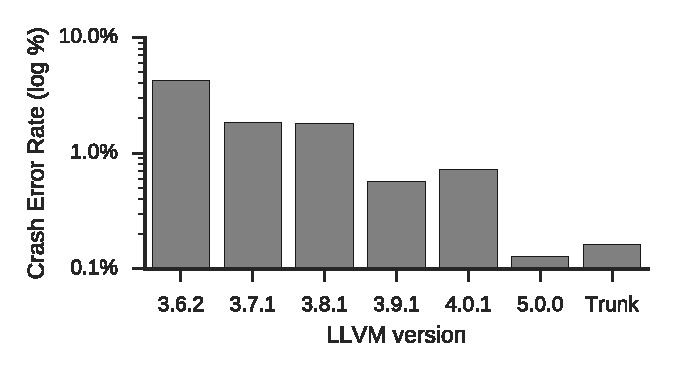
\includegraphics[width=.85\columnwidth]{img/clang-crashes}%
  \caption[Crash rate of the Clang front-end]{%
    Crash rate of the Clang front-end of every LLVM release in the past 24 months compiling 75k DeepSmith kernels.%
  }%
  \label{fig:clang-clash-rate}
\end{figure}

\begin{table}
  \centering %
  \begin{tabular}{r|ccccccc}
  \toprule
  {} & 3.6.2 & 3.7.1 & 3.8.1 & 3.9.1 & 4.0.1 & 5.0.0 & Trunk \\
  \midrule
  Assertion 1 & 2962 & 1327 & 1332 & 414 & 523 & 83 & 97 \\
  Assertion 2 & & 1 & 1 & & & &       \\
  Assertion 3 & & & & & & & 1 \\
  Assertion 4 & & & & & & & 2 \\
  Assertion 5 & 147 & & & & & &       \\
  Assertion 6 & 1 & & & & & &       \\
  Assertion 7 & & & & 1 & 1 & &       \\
  Unreachable & 86 & 42 & 14 & 14 & 18 & 13 & 21 \\
  \bottomrule
\end{tabular}

  \caption[Number of DeepSmith programs which trigger errors]{%
    The number of DeepSmith programs which trigger distinct Clang front-end assertions, and the number of programs which trigger unreachables.%
  }
  \label{tab:clang-crash-rate}
\end{table}

The results emphasise that compiler validation is a moving target. Every change and feature addition has the potential to introduce regressions or new failure cases. Since LLVM will not release unless their compiler passes their own extensive test suites, this also reinforces the case for compiler fuzzing. DeepSmith provides an effective means for the generation of such fuzzers, at a fraction of the cost of existing techniques.


\subsection{Extensibility of Language Model}
\label{subsec:deepsmith-solidity-extensibility}

\begin{table}
  \centering %
  \caption{%
    The number of DeepSmith programs that trigger Solidity compiler crashes in 12 hours of testing.%
  }
  \begin{tabular}{|rc|ccc|}
    \hline
    \rowcolor{gray!50}
    \textbf{Compiler} & $\pm$ & \textbf{Silent Crashes} & \textbf{Assertion 1} & \textbf{Assertion 2}\\
    \multirow{ 2}{*}{solc}    & $-$ & 204 & 1 & \\
    & $+$ & 204 & 1 & \\
    \rowcolor{gray!25}
    & $-$ & 3628 & 1 & 1\\
    \rowcolor{gray!25}
    \multirow{ -2}{*}{solc-js} & $+$ & 908 & 1 & 1\\
    \hline
  \end{tabular}
  \label{tab:preliminary-solidity-results}
\end{table}


A large portion of the DeepSmith architecture is language-agnostic, requiring only a corpus, encoder, and harness for each new language. This potentially significantly lowers the barrier-to-entry compared with prior grammar-based fuzzers. This section reports on initial results in extending DeepSmith to the Solidity programming language. Solidity is the smart contract programming language of the Ethereum blockchain. At less than four years old, it lacks much of the tooling of more established programming languages. Yet, it is an important candidate for rigorous testing, as exploitable bugs may undermine the integrity of the blockchain and lead to fraudulent transactions.


\subsubsection{Testing Methodology}

The same methodology was applied to train the program generator as for OpenCL. A corpus of Solidity contracts was assembled from GitHub, recursively inlining imported modules where possible. The same tokeniser was used as for OpenCL, only changing the list of language keywords and builtins. Code style was enforced using clang-format. The model is trained in the same manner as OpenCL. No modification to either the language model or generator code was required. A simple compile-only test harness is used to drive the generated Solidity contracts.


\subsubsection{Initial Results}

The generator and harness loop was run for 12 hours on four testbeds: the Solidity reference compiler \texttt{solc} with optimisations on or off, and \texttt{solc-js}, which is an Emscripten compiled version of the \texttt{solc} compiler. Table~\ref{tab:preliminary-solidity-results} summarises the results. Numerous cases were found where the compiler silently crashes, and two distinct compiler assertions. The first is caused by missing error handling of language features (this issue is known to the developers). The source of the second assertion is the JavaScript runtime and is triggered only in the Emscripten version, suggesting an error in the automatic translation from LLVM to JavaScript.

Extending DeepSmith to a second programming required an additional 150 lines of code (18 lines for the generator and encoder, the remainder for the test harness) and took about a day. Given the re-usability of the core DeepSmith components, there is a diminishing cost with the addition of each new language. For example, the OpenCL encoder and re-writer, implemented using LLVM, could be adapted to C with minimal changes. Given the low-cost of extensibility, these preliminary results indicate the utility of the approach for simplifying test case generation.
